
\newcommand{\fishfigwidth}{1.52in}

\begin{figure}
    \centering
    \begin{subfigure}[t]{\fishfigwidth}
        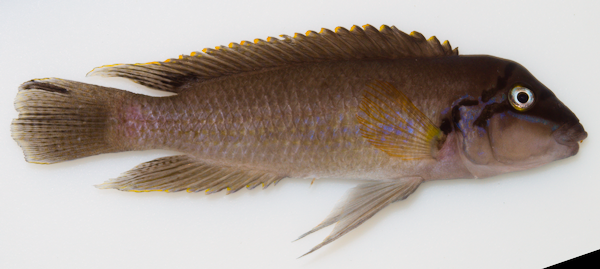
\includegraphics[width=\fishfigwidth]{FishPoo/figures/host_phenotypes/Chalinochromis_brichardi}
        \small
        \caption{\textit{Chalinochromis brichardi}}
    \end{subfigure}
    \begin{subfigure}[t]{\fishfigwidth}
        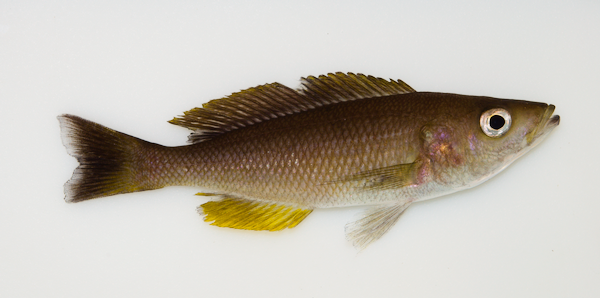
\includegraphics[width=\fishfigwidth]{FishPoo/figures/host_phenotypes/Cyprichromis_coloratus}
        \small
        \caption{\textit{Cyprichromis coloratus}}
    \end{subfigure}
    \begin{subfigure}[t]{\fishfigwidth}
        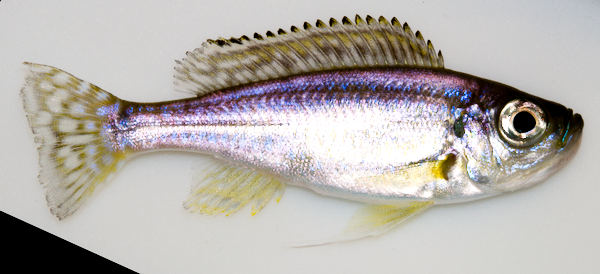
\includegraphics[width=\fishfigwidth]{FishPoo/figures/host_phenotypes/Haplotaxodon_microlepis}
        \small
        \caption{\textit{Haplotaxodon microlepis}}
    \end{subfigure}
    \begin{subfigure}[t]{\fishfigwidth}
        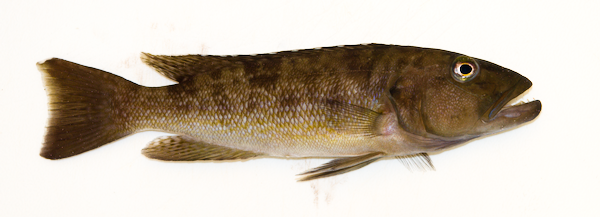
\includegraphics[width=\fishfigwidth]{FishPoo/figures/host_phenotypes/Lepidiolamprologus_profundicola}
        \small
        \caption{\textit{Lepidiolamprologus profundicola}} 
    \end{subfigure} \\
    \begin{subfigure}[t]{\fishfigwidth}
        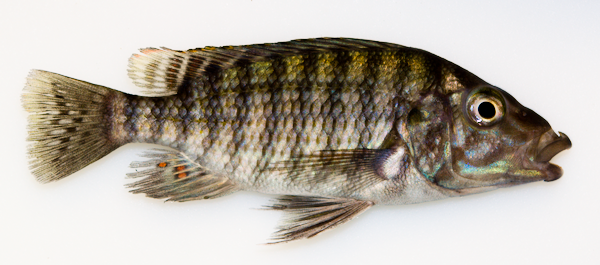
\includegraphics[width=\fishfigwidth]{FishPoo/figures/host_phenotypes/Lobochilotes_labiatus}
        \small
        \caption{\textit{Lobochilotes labiatus}}
    \end{subfigure}
    \begin{subfigure}[t]{\fishfigwidth}
        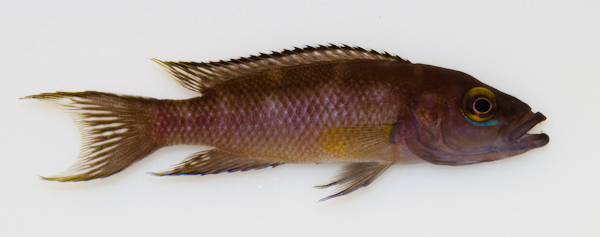
\includegraphics[width=\fishfigwidth]{FishPoo/figures/host_phenotypes/Neolamprologus_buescheri}
        \small
        \caption{\textit{Neolamprologus buescheri}}
    \end{subfigure}
    \begin{subfigure}[t]{\fishfigwidth}
        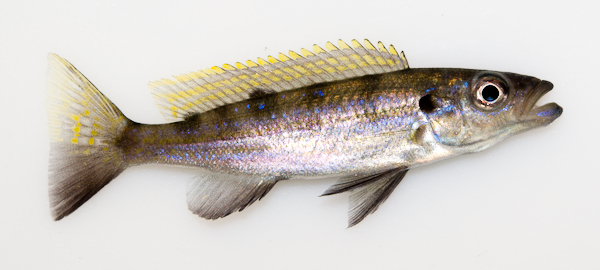
\includegraphics[width=\fishfigwidth]{FishPoo/figures/host_phenotypes/Perissodus_microlepis}
        \small
        \caption{\textit{Perissodus microlepis}}
    \end{subfigure}
    \begin{subfigure}[t]{\fishfigwidth}
        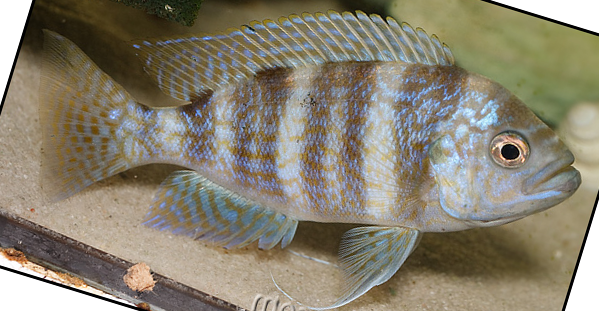
\includegraphics[width=\fishfigwidth]{FishPoo/figures/host_phenotypes/Plecodus_straeleni}
        \small
        \caption{\textit{Plecodus straeleni}} 
    \end{subfigure} \\
    \begin{subfigure}[t]{\fishfigwidth}
        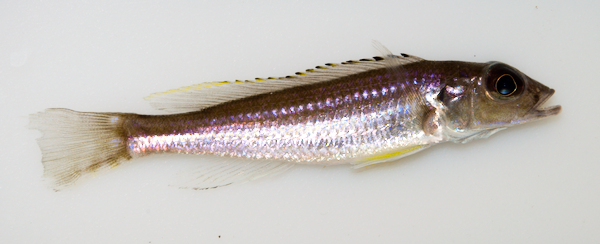
\includegraphics[width=\fishfigwidth]{FishPoo/figures/host_phenotypes/Reganochromis_calliurus}
        \small
        \caption{\textit{Reganochromis calliurus}}
    \end{subfigure}
    \begin{subfigure}[t]{\fishfigwidth}
        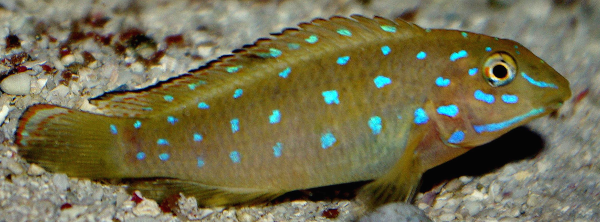
\includegraphics[width=\fishfigwidth]{FishPoo/figures/host_phenotypes/Tanganicodus_irsacae}
        \small
        \caption{\textit{Tanganicodus irsacae}}
    \end{subfigure}
    \begin{subfigure}[t]{\fishfigwidth}
        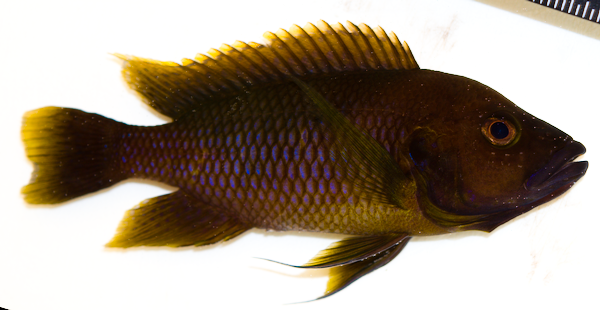
\includegraphics[width=\fishfigwidth]{FishPoo/figures/host_phenotypes/Trematochromis_benthicola_large}
        \small
        \caption{\textit{Trematochromis benthicola}}
    \end{subfigure}
    \begin{subfigure}[t]{\fishfigwidth}
        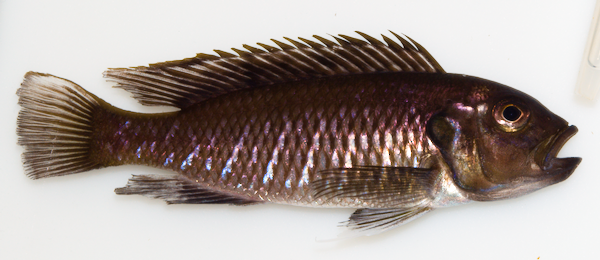
\includegraphics[width=\fishfigwidth]{FishPoo/figures/host_phenotypes/Triglachromis_otostigma}
        \small
        \caption{\textit{Triglachromis otostigma}} 
    \end{subfigure} \\
    \begin{subfigure}[t]{\fishfigwidth}
        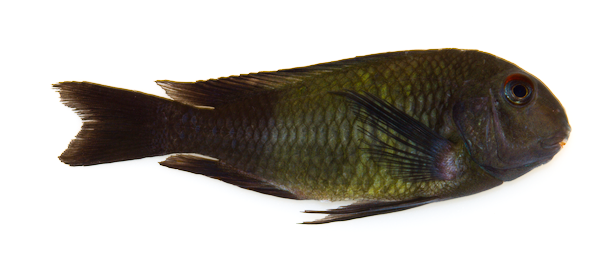
\includegraphics[width=\fishfigwidth]{FishPoo/figures/host_phenotypes/Tropheus_sp_black_Ikola}
        \small
        \caption{\textit{Tropheus} sp. black Ikola}
    \end{subfigure}
    \begin{subfigure}[t]{\fishfigwidth}
        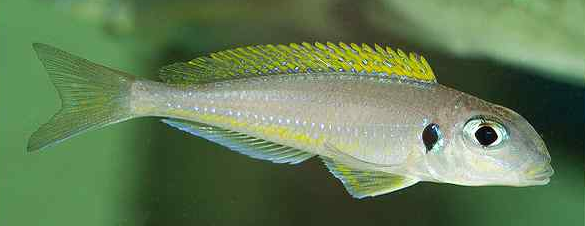
\includegraphics[width=\fishfigwidth]{FishPoo/figures/host_phenotypes/Xenotilapia_flavipinnis}
        \small
        \caption{\textit{Xenotilapia flavipinnis}}
    \end{subfigure}
    \caption{Live photographs of fishes used in this study (not to scale).}
    \label{FP_allfish}
\end{figure}

